\lfoot{Tobias Perny}

\begin{figure}[!htb]
	\centering
	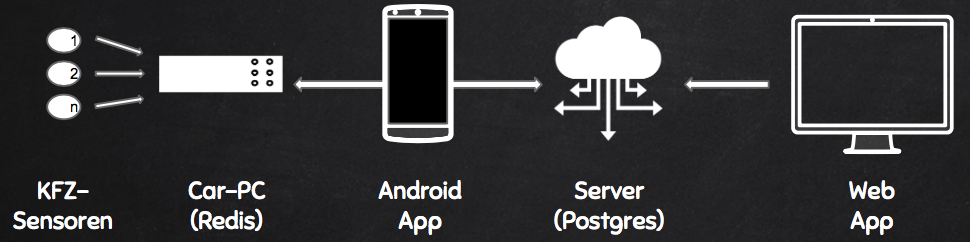
\includegraphics[scale=0.6]{images/konzept}
	\caption{Konzept des BestShift Systems}
\end{figure}

Zur Umsetzung dieses Projektes wurde eine Konzeptgrafik erstellt, um die Aufabentrennung zu visualisieren.
\nextline
Die erste Aufgabe ist das vergleichen und auswählen verschiedener Sensoren, mit welchen Beschleunigungskräfte und Innenraumtemperatur gemessen werden kann. Zu diesem Punkt zählt auch die Auswahl einen Bluetoothfähigen OBDII Adapters.
\nextline
Der nächste Punkt ist die Erstellung eines Car-PC's. Dieser muss in einen DIN-Schacht der Mittelkonsole eines Fahrzeugs installiert werden können. Auf diesem läuft ein Redis Server, und alle oben genannten Sensoren sind in diesem Integriert.
\nextline
Als weitere Komponente kann man auf obiger Grafik ein Smartphone erkennen, welches eine Android-Applikation symbolisiert. Mithilfe dieser Adroid-App kann der Fahrer seinen Fahrstil analysieren und möglicherweise verbessern.
\nextline
Zusätzlich dazu wird die Android App verwendet um die gesammelten Sensordaten auf unsere Server zu laden. Jegliche weitere Applikation kann sich dann vom Server die benötigte Information besorgen.
\nextline
Die Fokus der Web-App liegt bei der nachträglichen Analyse und dem Vergleich von mehreren Fahrten. Die benötigten Sensordaten werden vom Server bezogen. Zusätzlich dazu können auf der Web-App Einträge für soziallen Plattformen erstellt werden.